%\documentclass[graphics, twocolumn, usenatbib]{mn2e}
%\documentclass[twocolumn,iop,revtex4]{openjournal}
%\documentclass[linenumbers, twocolumn]{aastex631}
\documentclass[twocolumn, tighten]{aastex631}
%\usepackage[utf8]{inputenc}
%\usepackage{times}
\usepackage{natbib} 
%\usepackage{epsfig} 
%\usepackage{graphicx} 
%\usepackage[dvipsnames]{xcolor}
%\usepackage{deluxetable} 
\usepackage{aas_macros} 
\usepackage{amssymb}
\usepackage{amsmath}
\usepackage[title]{appendix}
\usepackage{hyperref}	% Hyperlinks
\hypersetup{colorlinks=true,linkcolor=blue,citecolor=blue,filecolor=blue,urlcolor=blue}
\usepackage[caption=false]{subfig}
%\usepackage{soul}                          % provides \hl{} for highlighting
\usepackage{ulem} \normalem 
%\usepackage{xifthen}
\newcommand{\lya}{Lyman-$\alpha$~}
\newcommand{\gad}{\textsc{Gadget-2~}}
\newcommand{\enzo}{\texttt{Enzo~}}
\newcommand{\enzoc}{\texttt{Enzo}}
\newcommand{\yt}{\texttt{yt~}}
\newcommand{\ytc}{\texttt{yt}}
\newcommand{\cloudy}{\texttt{Cloudy~}}
\newcommand{\grackle}{\texttt{Grackle-2.1~}}
\newcommand{\gracklec}{\texttt{Grackle-2.1}}
\newcommand{\enzolat}{\texttt{Enzo-2.3}}
\newcommand{\cosmos}{\textsc{Cosmos~}}

\newcommand{\darwin}{\textsc{Darwin~}}
\newcommand{\enzoamr}{\texttt{Enzo(AMR)~}}
\newcommand{\enzost}{\texttt{Enzo(static)~}}
\newcommand{\lyb}{Lyman-$\beta$~} 
\newcommand{\eg}{{\it e.g.~}}
\newcommand{\kms} {km $\rm{s^{-1}}$}
\newcommand{\mpch} {\rm $h^{-1}$ Mpc\,\,} 
\newcommand{\kpch} {\rm $h^{-1}$ kpc\,\,} 
\newcommand{\msolar} {$\rm{M_{\odot}}~$}
\newcommand{\msolarc} {$\rm{M_{\odot}}$}
%\newcommand{\msolaryr} {$\rm{M_{\odot}/yr}~$}
%\newcommand{\msolaryrc} {$\rm{M_{\odot}/yr}$}
\newcommand{\msolaryr} {$\rm{M_{\odot}~yr^{-1}}~$}
\newcommand{\msolaryrc} {$\rm{M_{\odot}~yr^{-1}}$}
\newcommand{\lsolar} {$\rm{L_{\odot}}~$}
\newcommand{\lsolarc} {$\rm{L_{\odot}}$}
\newcommand{\zsolar} {$\rm{Z_{\odot}}~$}
\newcommand{\zsolarc} {$\rm{Z_{\odot}}$}
\newcommand{\rsolar} {$\rm{R_{\odot}}~$}
\newcommand{\molH} {$\rm{H_2}$~}
\newcommand{\molHc} {$\rm{H_2}$}
\newcommand{\J} {$\rm{10^{-21}\ erg\ cm^{-2}\ s^{-1}\ Hz^{-1}\ sr^{-1}}$}
\newcommand{\inten} {$\rm{ erg\ cm^{-2}\ s^{-1}\ Hz^{-1}\ sr^{-1}}$~}
\newcommand{\JU} {$\rm{ erg\ cm^{-2}\ s^{-1}\ Hz^{-1}\ sr^{-1}}$}
\newcommand{\JLW} {J$_{\rm LW}$}
\newcommand{\healpix} {\texttt{HEALPix~}}
\newcommand{\smartstar} {\texttt{SmartStar~}}
\newcommand{\smartstars} {\texttt{SmartStars~}}
\newcommand{\smartstarsc} {\texttt{SmartStars}}
\newcommand{\smartstarc} {\texttt{SmartStar}}
\newcommand{\rarepeak} {\textit{Rarepeak~}}
\newcommand{\rarepeakc} {\textit{Rarepeak}}
\newcommand{\normal} {\textit{Normal~}}
\newcommand{\normalc} {\textit{Normal}}
\newcommand{\void} {\textit{Void~}}
\newcommand{\voidc} {\textit{Void}}
\newcommand{\ha} {\texttt{HaloA~}}
\newcommand{\hb} {\texttt{HaloB~}}
\newcommand{\hac} {\texttt{HaloA}}
\newcommand{\hbc} {\texttt{HaloB}}

\def\jr#1{{\color{orange} \bf JR:  #1}}

\newcommand{\note}[1]{{\noindent\hspace{-3em}\bf\color{Plum}$\longrightarrow$ \quad{#1}}}
\newcommand{\delete}[1]{{\color{red}{\sout{#1}}}}
\newcommand{\change}[2][]{%
\ifthenelse{\isempty{#2}}{{\color{ForestGreen}{#1}}}%
{{\color{RedOrange}\sout{#1}}{\color{ForestGreen}{ #2}}}%
}


\def\majo#1{{\color{brown} \bf MJ:  #1}}

\submitjournal{ApJL}


\def\etal{{\it et al.}~}

\begin{document}
%\title[Leo I a fossil galaxy]{Is the dwarf galaxy Leo I a smoking gun for heavy massive black hole %seed formation?}
\title[Leo I a fossil galaxy]{Observational Signatures of Massive Black Hole Progenitor Pathways - Leo I as a Smoking Gun?}

\correspondingauthor{John Regan}
\email{john.regan@mu.ie}
\author[0000-0001-9072-6427]{John A. Regan}
\thanks{Royal Society - SFI University Research Fellow}
\affil{Department of Theoretical Physics, Maynooth University, Maynooth, Ireland}

\author{Fabio Pacucci$^{2}$}
\author{Maria Bustamanate$^{3}$ (Author order TBD)}





\begin{abstract}
 TBD
\end{abstract}

\keywords{Early Universe, Black Holes, Star Formation, Dwarf Galaxies, Numerical Methods}

\section{Introduction} \label{Sec:Introduction}
\noindent Super Massive Black Holes with masses greater than $10^6$ \msolar are routinely observed in the centers of massive galaxies \citep[e.g.][]{Faber_1997, Marconi_2004, Heckman_2014} . In addition to this, there exists a strong correlation between the mass of the central massive black hole (MBH) and the velocity dispersion of stars in the central region of the host galaxy - the so-called $M-\sigma$ relation. This relation is particularly well understood empirically for black holes in the super massive range (M$_{BH} \gtrsim 10^6$ \msolarc) \cite[e.g.][]{Magorrian_1998, Kormendy_2013}. As observations are pushed to lower black hole masses in lower mass galaxies the relationship is less well defined both empirically and indeed theoretically. However, recent observations of dwarf galaxies by \cite{Baldassare_2020} in galaxies 
in the dwarf galaxy regime ($M_{*} \lesssim 5 \times 10^9$ \msolarc) have begun to extend the 
$M-\sigma$ into the dwarf galaxy mass range showing that the relation holds for black hole masses below the super massive black hole threshold. \\
\textcolor{red}{@Majo can up please edit these paragraphs on the observations. The first paragraph below I lifted from another recent paper by Fabio and me and needs to be edited for sure. }\\ 
\indent Black holes below the super massive black hole threshold are sometimes referred to as \textit{intermediate mass black holes} - rather than use this term in this paper we simply refer to all black holes with masses greater than 1000 \msolar as Massive Black Holes (MBHs). Black holes below this limit we will refer to as stellar mass black holes (although there is significant difficulty in applying concrete labels to black hole masses). Observations of MBHs in the dwarf galaxy regime are particularly challenging given that the black hole mass is observed to scale with the 
galaxy mass. As a result the sphere of influence of the (central) MBH is smaller relative to commensurate MBHs in more massive galaxies. Most searches of dwarf 
galaxies have focused on the use of optical narrow emission line diagnostic diagrams to identify active galactic nuclei (AGN) emission and of broad emission lines
to estimate the MBH mass \citep{Greene_2004, Greene_2007, Reines_2013, Moran_2014, Chilingarian_2018}. The use of optical variability and integral field spectroscopy 
(IFS) has yielded additional tens of hidden low-mass AGN whose emission is diluted by the star formation of the host galaxy. Most of these samples are however biased toward very local ($z < 0.3$) dwarf galaxies and are limited by obscuration. This has been circumvented by infrared, X-ray and radio searches of AGN in dwarf galaxies which has yielded the detection of AGN in dwarf galaxies out to $z \sim 3.4$. The use of wide and deep X-ray surveys has additionally provided a robust measurement of the number of AGN in dwarf galaxies out to $z \sim 0.7$. In almost all of these cases the mass of the accreting MBH comes from fitting the mass against the observed luminosity 
in the detection waveband. As a result there are inherent uncertainties to this approach. \\
\indent A more accurate measurement of the MBH mass comes when the kinematics of stars in close proximity to the MBH can be measured directly. Something about how in this case we can really drive down the uncertainty in the measurement of the central MBH. The recent discovery of a MBH with a mass of $ 3 \times 10^6$ \msolar in the dwarf spheroidal galaxy Leo I was achieved using such a method....
\majo{more than more accurate, it's a clean independent probe that works only for nearby dwarfs, in which you can resolve the central parsecs. Dwarfs nearby are mostly gas depleted, so there's not really any alternative probe available....} \jr{Ok cool. Could you update this section with that info fleshed out a bit more? Thanks!}
\\ \\
MBH seeding is expected to be initiated at high redshift ($z \gtrsim 10$) in galaxies which are either of primordial composition or near-primordial composition. 
The nature of the MBH seed is then of central importance. MBH seeds can be broken down into either \textit{light} or \textit{heavy} seeds. Light seeds are expected to be produced in abundance by the first generation of metalfree stars with typical masses in the range 10 - 100 \msolarc \citep[e.g.][]{Turk_2012, Stacy_2016}. However, the distribution of end point masses of the 
first stars is likely to have a tail to several hundred solar masses \citep[e.g.][]{Hirano_2014}. Starting from these \textit{light} seeds these stellar mass black holes would need to grow by approximately 3 orders of magnitude in order to become sufficiently massive that they could settle at the centre of even a dwarf galaxy \citep{Pfister_2019}. Heavy seeds on the other hand are speculated to form in more massive haloes where star formation is initially suppressed \citep{Loeb_2001, Haiman_2006, Volonteri_2012}. The suppression of star formation as the halo grows means that
the Jeans mass of the (gravitationally) unstable gas is increased which then favours the formation of more massive stars. Three mainstream mechanisms have been identified through 
which environments for \textit{heavy} seed star formation can occur. \\
\indent Firstly, the Lyman-Werner (LW) flux from a neighbouring massive galaxy may be sufficient to sterilise the host galaxy of \molH \citep{Dijkstra_2008, Dijkstra_2014, Visbal_2014, Regan_2017}. \molH can cool the gas in
early galaxies down to approximately 200 K and is the main coolant through which the first stars form. Removing this pathway leaves the gas unable to cool and 
suppresses star formation. Secondly, the rapid assembly of a dark matter halo can lead to a situation where the dynamical heating induced by the rapid assembly 
exceeds the energy lost through \molH cooling \citep{Yoshida_2003a, Fernandez_2014, Wise_2019, Regan_2020b}. In this case star formation is again suppressed - at least until cooling by atomic Hydrogen becomes important above approximately 8000 K \citep{Omukai_2001}. Thirdly, the velocity offset between baryons and dark matter following recombination can introduce a delay in the settling of gas in the centre of assembling dark matter haloes - this is referred to as dark matter streaming \citep{Tseliakhovich_2010}. The time delay means that the dark matter halo is more 
massive before the gas can virialise and this in turn leads to a larger Jeans mass and again more massive stars \citep{Tanaka_2014, Hirano_2017, Schauer_2017, Latif_2014c, Kulkarni_2021}.\\
\indent Following seeding MBHs grow through mergers and accretion. However, evidence of the seeding process of MBHs in galaxies is expected to be erased leaving no clear signature of the seed mass or seed formation pathway. In this paper we argue that there may be a mechanism through which we can use some indirect evidence within fossil dwarf galaxies to differentiate between \textit{light} seed and \textit{heavy} seed progenitors. Fossil dwarf galaxies are dwarf galaxies found in the present day universe but which initially formed in the very early Universe and have not yet being merged into more galaxies. \\
\indent Fossil dwarf galaxies have been highlighted previously in the literature as key environments in which to test models of early MBH formation \citep[e.g][]{Volonteri_2008, VanWassenhove_2010}. However, even when a central MBH is found in a fossil dwarf galaxy it's origin still cannot be cleanly ascertained. 
The premise of this paper is to highlight, based on analytical arguments and the results from high resolution MBH seeding simulations that a further signature of a \textit{heavy} seed channel
is the existence of a black hole continuum in mass from the stellar mass regime all the way up to the mass of the central MBH - see Fig. \ref{Fig:Cartoon}.
In \S $\ref{Sec:Model}$ we outline models for MBH growth through both the \textit{light} and \textit{heavy} seed channels showing how the different pathways may be distinguished given sufficiently sensitive observations
of MBH demographics in fossil dwarf galaxies. In \S \ref{Sec:LeoI} 
we discuss the recent discovery of a $10^6$ \msolar mass black hole in the Leo I galaxy and argue that this galaxy is an ideal environment in which to test our model. 
In \S \ref{Sec:Discussion} we discuss the implications of our postulates and in \S \ref{Sec:Conclusions} we give our conclusions. 


%%%%%%%%%%%%%%%%%%%%%%%%%%%%%%%%%%%%%%%%%%%%%%%%%%%%%%%%%%%%%%%%%%%%%%%%%%%%%%
%%%%%%%%%%%%%%%%%%%%%%%%%%Figure 1%%%%%%%%%%%%%%%%%%%%%%%%%%%%%%%%%%%%%%%%%%%%%
\begin{figure*}
\centering
\begin{minipage}{175mm}      \begin{center}
\centerline{
    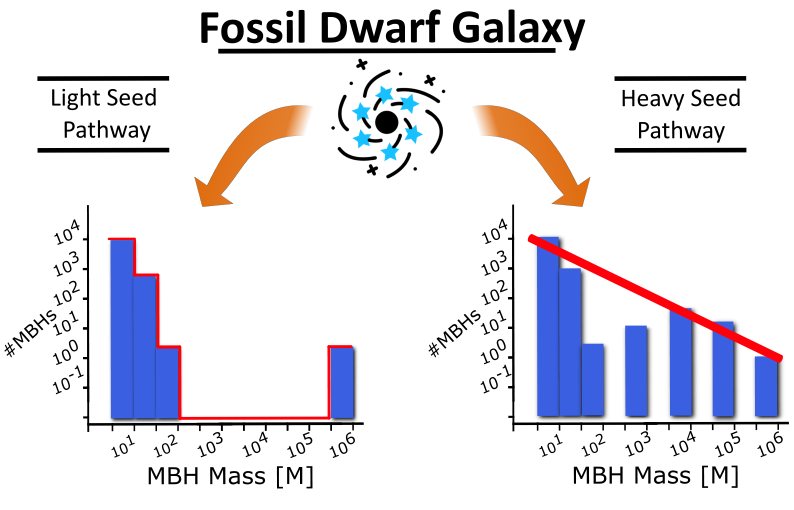
\includegraphics[width=18.0cm, height=14cm]{Figure1.3.png}}
\caption{\textbf{This diagram is currently awful I know! This is just a sketch. A much improved version will appear here soon!} The spectrum of black hole masses inside a fossil dwarf galaxy. For the \textit{light} seed pathway only one (central) massive black hole is expected with a 
gap between the mass of the central black hole and that of the stellar remnant black holes that will populate the galaxy. For the \textit{heavy} seed channel on the other-hand a 
black hole mas continuum is expected as the gas initially fragments during the initial seeding process leaving behind a number of \textit{heavy} seed fragments. While some of the 
fragments will merge with the central objects - other fragments will remain in the core of the galaxy as passive MBHs.}
\label{Fig:Cartoon}
\end{center} \end{minipage}
\end{figure*}
%%%%%%%%%%%%%%%%%%%%%%%%%%%%%%%%%%%%%%%%%%%%%%%%%%%%%%%%%%%%%%%%%%%%%%%%%%%%%%%%%%
\section{Model} \label{Sec:Model}
\noindent Our model for determining the progenitor seeds of MBHs leverages two underlying assumptions, both of which are based on results in the literature and 
furthermore quantified by analytical models. In addition our model is restricted to the dwarf 
galaxy regime and does not apply to galaxies which have grown beyond this mass scale. 

\begin{enumerate}
    \item We assume that if \textit{light} seeds are the progenitors of MBHs then this relies on the spectacular growth of a single light seed and that the probability of multiple \textit{light} seeds undergoing rapid growth within a single (dwarf) galaxy is remote. A number of independent investigations spanning more than a decade \citep{Volonteri_2008, Alvarez_2009, Milosavljevic_2009, Jeon_2012, Smith_2018} have all reached broadly similar conclusions - that stellar mass black holes seeded within cosmological environments do not grow appreciably (if at all) in dwarf galaxies. 
    \item We assume that \textit{heavy seeds} are formed with masses in the range $M_{\rm{seed}} = 10^3 - 10^5$ \msolarc. These \textit{heavy} seed masses are consistent with the range of masses found by a number of independent recent studies \cite[][]{Regan_2017, Latif_2014a, Regan_2020b}. Furthermore, given that avoiding fragmentation appears extremely difficult to achieve \citep{Regan_2018a}, we assume that fragmentation is a ubiquitous occurrence and that numerous \textit{heavy} seeds with masses in the range $M_{\rm{seed}} = 10^3 - 10^5$ \msolar are created.
\end{enumerate}

\noindent We now begin by analysing our two underlying assumptions in detail.\\

\noindent Population III stars are the first generation of stars born out of primordial Hydrogen and Helium. As the first stars end their lives they will inevitably form black holes with masses that 
are expected to be comparable to their final stellar mass \citep{Heger_2003}. Similar to massive star formation in the present day, PopIII stars are expected to be born in multiples \citep{Clark_2008, Turk_2009, Clark_2011, Clark_2011a} and thus even mini-haloes are expected to host a number of massive stars. The remnant black holes left behind from PopIII stars have in the past been invoked as possible progenitors of MBHs \citep{Madau_2001}. However, both semi-analytic models and numerical simulations which have attempted to model the growth of PopIII remnant black holes over cosmic time have consistently showed that these \textit{light} seeds do not grow \citep{Volonteri_2008, Alvarez_2009, Smith_2018}.\\
\indent \textit{Light} seed growth has been shown to be possible within more idealised settings - particularly where a \textit{light} seed is able to accrete within the confines of a 
dense stellar cluster \citep[e.g.][]{Alexander_2014, Natarajan_2021} or within a circum-nuclear disk \citep{Lupi_2016}. However, while such conditions are possible, no cosmological
simulations have being able to show \textit{light} seed growth within such systems and hence no self-consistent modelling of this scenario exists as of yet. Also, and of particular relevance to this paper - such setups are not found in low mass dwarf galaxies within which the gravitational well is simply too small to host such dense stellar and/or gas 
environments. As a result our assumption
that \textit{light} seeds are extremely unlikely to grow within dwarf galaxies is well founded. \\
\indent However, we cannot exclude the possibility of \textit{light} seed rapid growth. It is possible that one PopIII remnant black hole, through random chance, is able to grow rapidly perhaps by finding itself continually, or at least frequently enough, at the centre of a converging flow gaining enough mass to settle at the centre of the dark matter halo \citep{Pfister_2019}. We quantify the probability of a PopIII remnant black hole growing through accretion in the core of a galaxy as follows:
We first assume that the mass of the PopIII remnant is 500 \msolar (which is in itself an optimistic assumption) giving a Bondi-Hoyle radius (from which a cross section can be calculated) of $R_{bondi} \sim 1 \times 10^{-2}$ pc. In order to calculate the probability that a PopIII remnant black hole intersects, or finds itself at the centre of a sufficiently dense gas cloud, we calculate first the probability, $P_{BH\_in\_cloud}$, that a black hole is in a sufficiently dense volume relative to the volume of the galactic core
\begin{equation}
\rm{P_{BH\_in\_cloud} = (R_{cloud}/R_{galcore})^3}
\end{equation}
where $R_{cloud}$ is the radius of the gas cloud and $R_{galcore}$ is the radius of the core of galaxy. We set $R_{cloud} = 0.1$ pc and $R_{galcore} = 20$ pc. Both of 
these values are chosen (and are highly conservative) based on high-z simulation results from \cite{Regan_2020b}. We multiply this number by the number of clouds expected in this region. For this we assume that $1 \times 10^{-4}$ (1 \% by volume) of  $R_{galcore}$ is filled with sufficiently dense gas giving $N_{clouds} \sim 800$. $N_{clouds}$ is therefore the number of gas clouds at any one time inside the galactic core each of which are expected to 
allow black hole growth. Finally, we compute, assuming that the 
black hole walks a random trajectory around that galaxy that the fraction of the volume sampled by the black hole, $V_{sampled}$, in a Hubble time, $\tau_{Hubble}$, is given by 
\begin{equation}
    \rm{V_{\rm{sampled}} = {{\tau_{Hubble} R_{bondi}^2 v_{BH}} \over {2 R_{galcore}^3}}}
\end{equation}
\iffalse
\begin{equation}
   \majo{ V_{sampled} = \frac{3}{4}\frac{R_{bondi}^2}{R_{galcore}^3}\tau_{Hubble}  v_{BH} }
   \tag{\majo{This is unitless, 
   but I'm not sure if it's the same idea.}}
\end{equation}
\fi
where $v_{BH}$ is the average relative velocity of the black hole (set here to be equal to the sound speed of the gas $\sim 10$ \kms). The total probability of a PopIII remnant accreting within a high-z galaxy (for which these numbers are derived) is given by
\begin{equation} \label{probability}
    \rm{P_{growth} = P_{BH\_in\_cloud} * N_{clouds} * V_{sampled}}
\end{equation}
 Using the canonical set of values noted above Eqn \ref{probability} gives a probability that a 
 stellar mass black holes intersects a single dense gas cloud within a Hubble time as, $P_{growth} \sim 9 \times 10^{-8}$.
 %\majo{$P_{growth} \sim 10^{-7}$ with the other equation, basically the same}. 
 This is quite an optimistic
 estimate given that we assume a large black hole mass for the PopIII remnant, we assume a large radius for the gas cloud size and we assume a small radius for the galactic core. Hence, this probabilistic estimate should be seen as an upper limit. We have neglected any treatment of dynamical friction in this estimate which is completely justified based on the mass of the black hole in this context \citep{Binney_1987}. Given this probability estimate the probability of two (or more) black holes within the same environment experiencing growth becomes infinitesimally small. It should also be noted that this calculation considers only the probability of the black hole encountering such an environment once when in fact a black hole more likely must encounter such an environment on multiple (perhaps hundreds of) occasions before the black hole becomes sufficiently massive that dynamical friction can act to bring the black hole to the centre of such a region and stabilise it there. \\

\indent Our assumptions on the mass of \textit{heavy} seeds are given by state-of-the-art cosmological simulations undertaken by numerous groups who agree that massive 
black hole seeds within the range $M_{\rm{seed}} = 10^3 $ - $M_{\rm{seed}} = 10^5$ are possible \citep{Hosokawa_2013, Latif_2013d, Regan_2014a, Inayoshi_2014, Inayoshi_2014b, Latif_2016a, Regan_2018a, Regan_2018b}. In idealised settings a single object (with masses up to $10^5$ \msolarc) can be formed \citep{Inayoshi_2014} but for models in which more cosmologically consistent treatments are performed the formation and retention of multiple fragments is either moderate \citep[e.g.][]{Regan_2018a, Regan_2018b} or more widespread \citep{Wise_2019, Regan_2020b}. While some of these fragments may eventually merge or be ejected from the 
halo it is also likely that many will survive either as isolated massive black holes or in stable binaries. Our postulate is, that left in the wake of the MBH that eventually settles to 
the centre of the galaxy, is a population of less massive fragments of the original formation sequence (see Figure \ref{Fig:Cartoon}). These fragments will themselves be MBHs in the range $M_{\rm{MBH}} = 10^3 - 10^5$. These MBH `leftovers' are the observational
signature of a \textit{heavy} black hole formation pathway in (fossil) dwarf galaxies. This model does not apply to 
more massive galaxies in which MBHs can be incorporated through subsequent mergers over cosmic time and is valid only in fossil dwarf galaxies. 
We quantify this mechanism using the following model:\\ \\


\textcolor{red}{Just a few notes of a simple model. Note that this model can be used iteratively, as I explain at the end.}

We call $M_{\bullet, f}$ the final mass of the black hole in the galaxy. In our case, $M_{\bullet, f} = 3\times 10^6 M_\odot$. We can call $M_{\bullet, s}$ the mass of the single-mass population of seeds. This can be a light seed mass or a heavy seed mass. We call $\cal{A}$ the percent increase of mass of each black hole seed achieved by accretion. In the case of Leo I, probably $\cal{A} \sim 1$, as there was not much gas. Finally, we call $N_{mm}$ the number of seeds that must merge (MM) to reach the final mass $M_{\bullet, f}$. We can write:
\begin{equation}
    M_{\bullet, f} = M_{\bullet, s} \times A \times N_{mm}
\end{equation}
\textcolor{orange}{I would argue that this should be}
\begin{equation*}
    M_{\bullet, f} = M_{\bullet, s} \times N_{mm} + \sum_i A_i * M_{\bullet, s}i
\end{equation*}
\textcolor{orange}{- like you say though $A$ may well be negligible and we can neglect it. }
For example, if the final mass is 10 and accretion is negligible, and if you have seeds of 2 solar masses, $N_{mm} = 5$.
Of course, not all seeds will merge. The total number of seeds (of the single-mass population) is $N_{tot}$. Notably, $N_{tot} \geq N_{mm}$.
We call escape fraction $\varepsilon$ the fraction of the initial population of seeds that do not eventually merge to form the final SMBH, after an Hubble time. Of course $0 \leq \varepsilon \leq 1$. Specifically:
\begin{equation}
    N_{tot} = \frac{N_{mm}}{(1-\varepsilon)}
\end{equation}
The number of seeds that are left over (i.e., not end up part of the final BH) is $N_L = N_{tot} - N_{mm}$.
\begin{equation}
    N_L = N_{mm} \times \frac{\varepsilon}{(1-\varepsilon)}
\end{equation}
Note that if we can establish that:
\begin{equation}
    \varepsilon \propto M_{\bullet, s}^{-\alpha}
\end{equation}
with $\alpha > 0$, then the number of leftover black holes $N_L$ tends to zero as the mass of the initial seed increases.
So for very large BHs you don't expect a ``trail'' of smaller BHs.

\textcolor{red}{Note that we could devise an analytical way to do this iteratively. Think about starting with a population P1, some of them will merge and some of them will be left out, then we reach population P2 etc etc... I think we could find some finite series to establish some sort of power law of the mass distribution...}


\section{The Massive Black Hole in the Dwarf Galaxy \textit{Leo I}} \label{Sec:LeoI}
\noindent \textcolor{red}{Over to you @Majo!}
The recent observation of a MBH at the centre of dwarf spheroidal galaxy Leo I by \cite{Bustamante-Rosell_2021} represents one of the most massive black holes found at the centre of
a dwarf galaxy. Its mass was estimated at M$_{MBH} = (3.3 \pm 2) \times 10^6$ \msolar lifting
it significantly above the standard M$_{MBH} - \sigma$ relation \citep{Kormendy_2013, Baldassare_2020, Greene_2020} for both very massive and dwarf galaxies alike. 
@Majo perhaps you could write a few sentences/paragraphs here on the discovery (crowding etc) and on the 
confidence with which you have in the result (i.e. the 95\% confidence)


\section{Discussion \& Future Observational Markers} \label{Sec:Discussion}
\noindent The discovery of a $10^6$ \msolar at the centre of the dwarf spheroidal galaxy Leo I is an intriguing
observation. Leo I has an estimated virial mass of M$_{vir} = (7 \pm 1) \times 10^8$ \msolar \citep{McConnachie_2012} and a stellar mass of M$_{*} = 5.5 \times 10^6$ \msolar \citep{Mateo_2008}. 
With a central black hole mass of M$_{MBH} = (3.3 \pm 2) \times 10^6$ \msolar \citep{Bustamante-Rosell_2021} this black hole is significantly overmassive (by approximately a factor of $10^3$) compared to the virial mass of the halo. What does this mean for the 
formation pathways of the central MBH?\\
\indent Numerous authors have argued that satellite galaxies, irradiated by a nearby massive galaxies, will host obese 
massive black holes \citep{Agarwal_2013, Natarajan_2017, Scoggins_2022} formed via the \textit{heavy} seed paradigm in which
super-massive stars are a potential intermediate stage. For the case of Leo I the \textit{heavy} seed formation pathway
may have been induced via either a intense burst of Lyman-Werner radiation, the rapid assembly of 
the original Leo I galaxy component, baryonic streaming velocities - or a combination of 
one of more of these mechanisms. In either case the result is broadly similar - a small number 
of massive black holes are expected to form in the centre of the embryonic dwarf galaxy - Leo I in this case. \\
\indent Dwarf galaxies have long been noted as potential sites in which to search for the fossils 
of the very early stages of MBH formation \citep{Volonteri_2008, VanWassenhove_2010}. We 
extend that idea here by also postulating that a specific observational signature of \textit{heavy} seed
MBH formation would be the existence of a continuum in mass of MBHs from the stellar mass all the way up to the mass of the central MBH. 
We illustrate this methodology and its outcome in Figure \ref{Fig:Cartoon}. If the seed for the central MBH was a light seed then no such continuum should exist
and there should be a clear gap in the black hole mass spectrum in fossil dwarf galaxies between the mass of the most massive black hole in the galaxy and the 
population of stellar mass black holes. \\
\indent What we are postulating here is that there will be evidence of the seeding mechanism in the black hole mass 
spectrum of the dwarf galaxy and that this signature may survive to the 
present day. While the black holes themselves carry no information of their accretion or merger history that is easily disentangled there may be clues 
from the black hole demographics inside fossil dwarf galaxies like Leo I. Fragmentation, even in the \textit{heavy} seed formation channel, is a 
robust prediction. As we demonstrate in \S \ref{Sec:Model} at least some of the original 
massive black holes will survive as isolated or binary massive black holes. It is these 
left over massive black holes, with masses less than that of the central massive black hole 
that we postulate to be observational signatures of a \textit{heavy} seed formation scenario. \\
\indent It is important to note that the 
absence of a continuum of black hole masses does not by itself falsify the \textit{heavy} seed scenario (as either mergers, ejections or very low levels of fragmentation could equally be 
responsible) but instead that the observation of a black hole mass spectrum would be strong evidence for a \textit{heavy} seed formation channel. We encourage further in depth observations 
and modelling of the dynamics inside Leo I as an environment in which to probe MBH seeding channels. 


\section{Conclusions} \label{Sec:Conclusions}

%====================================================================
\section*{Acknowledgements}
%====================================================================

\noindent JR acknowledges support from the Royal Society and Science Foundation Ireland under
grant number URF$\backslash$R1$\backslash$191132. JR also thanks the organisers of the 
\textsc{Intermediate Mass Black Holes: New Science from Stellar Evolution to Cosmology} 
during which the concept for this paper was born.

\label{lastpage}
\bibliographystyle{mn2e}
\bibliography{mybib}
\end{document}


